%%%%%%%%%%%%%%%%%%%%%%%%%%%%%%%%%%%%%%%%%%%%%%%%%%%%%%%%%%%%%%%%%%%%%%%%%%%%%%%%
\chapter{Реализация алгоритма}
\label{chap:impl}
%%%%%%%%%%%%%%%%%%%%%%%%%%%%%%%%%%%%%%%%%%%%%%%%%%%%%%%%%%%%%%%%%%%%%%%%%%%%%%%%

Для оценивания эффективности предложенного в разделе~\ref{chap:dev} решения, реализауем его в виде программной библиотеки (реализация алгоритма). Результаты, полученные с помощью данной реализации будут использованы в разделе~\ref{chap:quality} для проведения экспертного анализа.

В данном разделе рассматриваются некоторые аспекты реализации описанного алгоритма извлечения ВОП из обращений в службу поддержки, описана структура проекта, определены используемые технологии. Исходный код реализации алгоритма доступен на прилагаемом к данной работе CD-диске.

%%%%%%%%%%%%%%%%%%%%%%%%%%%%%%%%%%%%%%%%%%%%%%%%%%%%%%%%%%%%%%%%%%%%%%%%%%%%%%%%
\section{Используемые технологии}
%%%%%%%%%%%%%%%%%%%%%%%%%%%%%%%%%%%%%%%%%%%%%%%%%%%%%%%%%%%%%%%%%%%%%%%%%%%%%%%%
Для реализации алгоритма использовались следующие технологии: Java, Kotlin, Gradle, Git, JUnit, MongoDB, Mallet.

В качестве языка программирования используется \textit{Kotlin}. Kotlin~--- это активно развивающийся язык программирования общего назначения для JVM, к достоинствам которого относятся:

\nomenclature{JVM}{Java Virtual Machine}

\begin{itemize*}
\item Вывод типов;
\item Статическая типизация;
\item Мультипарадигменность;
\item Nullable типы данных;
\item Выразительный синтаксис;
\item Совместимость с java кодом.
\end{itemize*}

Описанные выше достоинста языка позволяют решать поставленные перед программистом задачи более эффективно, чем при использовании java. При этом, благодаря совместимости с java, сохраняется возможность исползования большого количества существующих java-библиотек.

На момент написания данной работы, Kotlin поддерживает Gradle, Maven и Ant для автоматической сборки проектов. \textit{Gradle}~--- система автоматической сборки, предоставляющая DSL на языке Groovy, и, по сравнению с другими решениями, использующими XML, позволяет писать более компактные сценарии сборки.

\nomenclature{DSL}{Domain-Specific Language, Предметно-ориентированный язык}
\nomenclature{XML}{eXtensible Markup Language}
\nomenclature{JSON}{JavaScript Object Notation}
\nomenclature{СУБД}{Система Управления Базами Данных}

\textit{Git}~--- система контроля версий, используемая командой YouTrack.

\textit{JUnit}~--- библиотека для модульного тестирования программного обеспечения. Совместима с Kotlin.

Для хранения данных используется \textit{MongoDB}. Для работы с обращениями в службу поддержки команда YouTrack использует Zendesk. Загружаемые из Zendesk данные имеют JSON формат. Поскольку MongoDB использует JSON-подобные документы и схему базы данных, было решено использовать данную СУБД, вместо реляционных баз данных.

\textit{Mallet}~\cite{MALLET}~--- библиотека на java, которая содержит реализацию необходимой тематической модели (LDA). Данная реализация написана в 2009 году, является наиболее 'взрослой' и развитой реализацией LDA. Подробнее о выборе реализации LDA написано в секции~\ref{sec:lda_choose}.

%%%%%%%%%%%%%%%%%%%%%%%%%%%%%%%%%%%%%%%%%%%%%%%%%%%%%%%%%%%%%%%%%%%%%%%%%%%%%%%%
\section{Структура проекта}
%%%%%%%%%%%%%%%%%%%%%%%%%%%%%%%%%%%%%%%%%%%%%%%%%%%%%%%%%%%%%%%%%%%%%%%%%%%%%%%%

Структура проекта представляет собой набор пакетов (\textit{packages}), каждый из которых соответсвует одному из этапов извлечения ВОП, описанными в разделе~\ref{chap:dev}. Общая структура пакетов предствалена на рисунке~\ref{fig:pckgs}. 

\begin{figure}[tph!]
\centerline{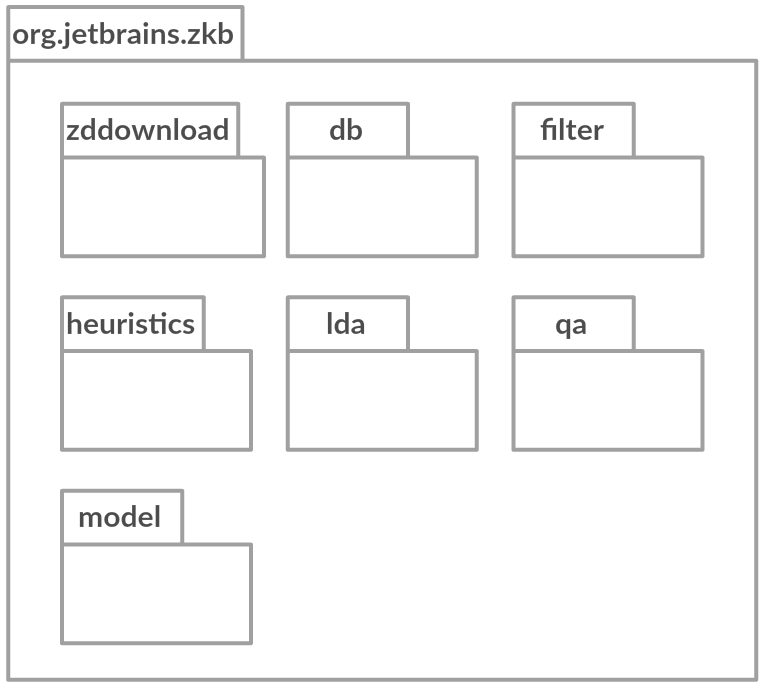
\includegraphics[width=7.5cm]{fig/pckgs.png}}
    \caption{Обобщенная структура пакетов реализации алгоритма}
    \label{fig:pckgs}
\end{figure}

Каждый из пакетов выполняет соответсвующую ему задачу:

\begin{itemize*}
\item org.jetbrains.zkb.zddownload~--- загрузка данных из Zendesk и сохранение их в базу данных;
\item org.jetbrains.zkb.db~--- данный пакет содержит классы отвечающие за зваимодействие с базой данных;
\item org.jetbrains.zkb.filter~--- содержит фильтры различного рода для анализируемых данных;
\item org.jetbrains.zkb.heuristics~--- эвристики предобработки;
\item org.jetbrains.zkb.lda~--- построение тематичечской модели анализируемых данных;
\item org.jetbrains.zkb.qa~--- формирование ВОП;
\item org.jetbrains.zkb.model~--- модель анализируемых данных, классы Ticket (обращение), Comment (комментарий) и так далее.
\end{itemize*}

Далее каждый из пакетов рассматривается более подробно.
%%%%%%%%%%%%%%%%%%%%%%%%%%%%%%%%%%%%%%%%%%%%%%%%%%%%%%%%%%%%%%%%%%%%%%%%%%%%%%%%
\section{Получение исходных данных}
%%%%%%%%%%%%%%%%%%%%%%%%%%%%%%%%%%%%%%%%%%%%%%%%%%%%%%%%%%%%%%%%%%%%%%%%%%%%%%%%

%%%%%%%%%%%%%%%%%%%%%%%%%%%%%%%%%%%%%%%%%%%%%%%%%%%%%%%%%%%%%%%%%%%%%%%%%%%%%%%%
\section{Взаимодействие с базой данных}
%%%%%%%%%%%%%%%%%%%%%%%%%%%%%%%%%%%%%%%%%%%%%%%%%%%%%%%%%%%%%%%%%%%%%%%%%%%%%%%%

%%%%%%%%%%%%%%%%%%%%%%%%%%%%%%%%%%%%%%%%%%%%%%%%%%%%%%%%%%%%%%%%%%%%%%%%%%%%%%%%
\section{Реализация предобработки данных}
%%%%%%%%%%%%%%%%%%%%%%%%%%%%%%%%%%%%%%%%%%%%%%%%%%%%%%%%%%%%%%%%%%%%%%%%%%%%%%%%
\subsection{Фильтрация данных}
\subsection{Эвристики предобработки}
%%%%%%%%%%%%%%%%%%%%%%%%%%%%%%%%%%%%%%%%%%%%%%%%%%%%%%%%%%%%%%%%%%%%%%%%%%%%%%%%
\section{построение тематической модели}
%%%%%%%%%%%%%%%%%%%%%%%%%%%%%%%%%%%%%%%%%%%%%%%%%%%%%%%%%%%%%%%%%%%%%%%%%%%%%%%%
\subsection{Выбор реализации LDA}
\label{sec:lda_choose}
%%%%%%%%%%%%%%%%%%%%%%%%%%%%%%%%%%%%%%%%%%%%%%%%%%%%%%%%%%%%%%%%%%%%%%%%%%%%%%%%
\section{Поиск вопросно-ответных пар}
%%%%%%%%%%%%%%%%%%%%%%%%%%%%%%%%%%%%%%%%%%%%%%%%%%%%%%%%%%%%%%%%%%%%%%%%%%%%%%%%

\Blindtext

  \begin{lstlisting}[language=Java, label={lst:aspectj_example}, 
  caption={Пример описания аспектов в AspectJ}]
aspect A  {
  pointcut fooPC(): execution(void Test.foo());
  pointcut printPC(): call(void System.out.println(String));
  
  before(): cflow(fooPC()) && printPC() {
    System.out.println("Hello, world!");
  }
}
  \end{lstlisting}

\lstinputlisting[
  label={listings:regexps_lnf},
  caption={Регулярные выражения для эвристик отображения},
  style={java}
]
{code/regexps_lnf.kt}

%%%%%%%%%%%%%%%%%%%%%%%%%%%%%%%%%%%%%%%%%%%%%%%%%%%%%%%%%%%%%%%%%%%%%%%%%%%%%%%%
\section{Резюме}
%%%%%%%%%%%%%%%%%%%%%%%%%%%%%%%%%%%%%%%%%%%%%%%%%%%%%%%%%%%%%%%%%%%%%%%%%%%%%%%%

\Blindtext
